% Standalone source for calibration dependency diagram.
% Build: cd figures && pdflatex calib-dependency.tex
% (Or: latexmk -pdf -cd figures/calib-dependency.tex)
\documentclass[tikz, border=3pt]{standalone}
\usetikzlibrary{positioning, arrows.meta, calc, bending, shapes.geometric, fit, backgrounds}
\tikzset{arr/.style={-{>[length=50pt, width=10pt, angle=60:5pt]}}}

\begin{document}
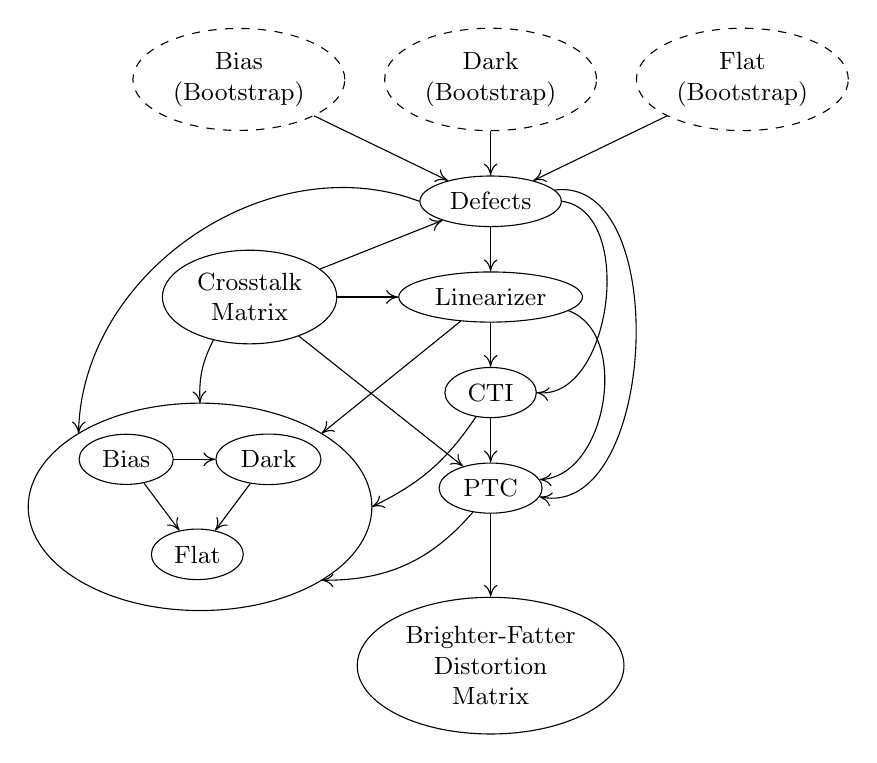
\begin{tikzpicture}[
      node distance=0.9em and 1.4em,
      every node/.style={draw, ellipse, align=center, font=\small},
      bootstrap/.style={dashed},
      every edge/.style={draw, arr},
      bend angle=15,
      feedback/.style={draw, arr, bend left=30, dashed},
      to box/.style={shorten >=0pt},
  ]
      % Top row: Bootstrap nodes (dashed borders)
      \node[bootstrap] (biasboot) {Bias\\(Bootstrap)};
      \node[bootstrap, right=of biasboot] (darkboot) {Dark\\(Bootstrap)};
      \node[bootstrap, right=of darkboot] (flatboot) {Flat\\(Bootstrap)};

      % Second row: Defects
      \node (defects) [below=1.6em of darkboot] {Defects};

      % Third row: Linearizer, Crosstalk
      \node (linearizer) [below=1.6em of defects] {Linearizer};
      \node (crosstalk) [left=2.2em of linearizer] {Crosstalk\\Matrix};

      % Fourth row: CTI, PTC
      \node (cti) [below=1.6em of linearizer] {CTI};
      \node (ptc) [below=1.6em of cti] {PTC};

      % Fifth row: Bias, Dark, Flat (triangle: Bias--Dark on top, Flat below center)
      \node (bias) [below left=4em and 1em of crosstalk] {Bias};
      \node (dark) [right=1.5em of bias] {Dark};
      \node (flat) [below=2.5em of $(bias)!0.5!(dark)$] {Flat};
      \node (bf) [below=3em of ptc] {Brighter-Fatter\\Distortion\\Matrix};

      % Box around Bias, Dark, Flat: fit node for arrow targets, draw box on background
      \node[draw, fit=(bias)(dark)(flat), inner sep=0em, outer sep=0pt] (calibbox) {};

      % Bootstrap -> Defects
      \draw[arr] (biasboot) -- (defects);
      \draw[arr] (darkboot) -- (defects);
      \draw[arr] (flatboot) -- (defects);

      % Defects -> Linearizer, CTI, PTC, and to calib box
      \draw[arr] (defects) -- (linearizer);
      \draw[arr] (defects) to[bend left=90] (cti);
      \draw[arr] (defects) to[bend left=100] (ptc);
      \draw[arr, to box] (defects.west) to[bend right=55] (calibbox.north west);

      % Linearizer -> CTI, PTC, and to calib box
      \draw[arr] (linearizer) -- (cti);
      \draw[arr] (linearizer) to[bend left=80] (ptc);
      \draw[arr, to box] (linearizer) -- (calibbox.north east);

      % Crosstalk -> Linearizer, PTC, and to calib box
      \draw[arr] (crosstalk) -- (linearizer);
      \draw[arr] (crosstalk) -- (ptc);
      \draw[arr] (crosstalk) -- (defects);
      \draw[arr, to box] (crosstalk) to[bend right=15] (calibbox.north);

      % CTI -> PTC, and to calib box
      \draw[arr] (cti) -- (ptc);
      \draw[arr, to box] (cti) to[bend left=15] (calibbox.east);

      % PTC -> Brighter-Fatter, and to calib box
      \draw[arr] (ptc) -- (bf);
      \draw[arr, to box] (ptc) to[bend left=25] (calibbox.south east);

      % Bias -> Dark, Flat
      \draw[arr] (bias) -- (dark);
      \draw[arr] (bias) -- (flat);
      \draw[arr] (dark) -- (flat);

\end{tikzpicture}
\end{document}
